\documentclass[11pt]{article}

% Packages
\usepackage[utf8]{inputenc}
\usepackage{amsmath, amssymb, amsthm}
\usepackage{enumitem}
\usepackage{geometry}
\usepackage{fancyhdr}
\usepackage{mathtools}
\usepackage{multicol}
\usepackage[colorlinks=true, urlcolor=blue, linkcolor=black, citecolor=black]{hyperref}

% Page layout
\geometry{margin=0.75in}
\pagestyle{fancy}
\fancyhf{}
\rhead{Ian Gallagher}
\lhead{Math 207C Homework}
\rfoot{\thepage}
\setlength{\headheight}{14pt}

% Commands
\newcommand{\vep}{\varepsilon}
\DeclarePairedDelimiter\abs{\lvert}{\rvert}

% Environments
\newtheoremstyle{problemstyle}
  {1em} % Space above
  {1em} % Space below
  {\normalfont} % Body font
  {} % Indent amount
  {\bfseries} % Theorem head font
  {} % Punctuation after theorem head
  {\newline} % Space after theorem head
  {} % Theorem head spec

\theoremstyle{problemstyle}
\newtheorem{problem}{Problem}

% Custom commands
\newenvironment{solution}
  {\noindent\textbf{Solution}\quad}
  {\hfill$\blacksquare$\par\vspace{1em}}

% Enumerate styles
\setlist[enumerate,1]{label=(\alph*), ref=\alph*, itemsep=0.2em, topsep=0.4em}
\setlist[enumerate,2]{label=(\roman*), ref=\roman*, itemsep=0.1em, topsep=0.2em}

% Title info
\title{Math 207C Homework \#\texttt{1}}
\author{Ian Gallagher}
\date{\today}

\begin{document}

\maketitle

\noindent Holmes Ex \#1.1, 1.3, 1.5, 1.7, 1.12, 1.18 (a)(e)(h)(p), 1.19, 1.20, 1.21

\begin{problem}[1.1]
\mbox{} % Add empty box to force a newline for the enumerate
\begin{enumerate}
  \item What values of $\alpha$, if any, yield 
        \(
        f = O\bigl(\vep^\alpha\bigr)
        \)
        as $\vep \downarrow 0$ for each of the following functions?
  \begin{multicols}{2}
    \begin{enumerate}
      \item $f = \sqrt{1 + \vep^2}$ 
      \item $f = \vep \sin(\vep)$ 
      \item $f = \bigl(1 - e^\vep\bigr)^{-1}$
      \item $f = \ln(1 + \vep)$
      \item $f = \vep \ln(\vep)$
      \item $f = \sin(1 / \vep)$
      \item $f = \sqrt{x + \vep}\text{, where } 0 \geq x \geq 1$ \newline\mbox{}
    \end{enumerate}
  \end{multicols}
\item For the functions listed in (a), what values of $\alpha$, if any, yield
      \(
      f = o\bigl(\vep^\alpha\bigr)
      \)
      as $\vep \downarrow 0$?
\end{enumerate}
\end{problem}

\begin{solution}
  \begin{enumerate}[label=(\roman*)]
    \item We can expand by plugging $x^2$ into the Taylor series for $\sqrt{1+x}$:
      \[ f = \sqrt{1 + \vep^2} = 1 + \frac{1}{2}\vep^2 - \frac{1}{8}\vep^4 + \cdots. \]
      Now, taking the ratio of limits we get,
      \[ \lim_{\vep \downarrow 0} \frac{f}{\vep^\alpha} = \lim_{\vep \downarrow 0}
        \left(\vep^{-\alpha} + \frac{1}{2}\vep^{2-\alpha} - \frac{1}{8}\vep^{4-\alpha} + \cdots \right) =
        \begin{cases}
          \infty, & \alpha > 0 \\
          1 , & \alpha = 0 \\
          0 , & \alpha < 0 
        \end{cases}\]
      Therefore, $f = O(\vep^\alpha)$ for $\alpha \leq 0$ and $f = o(\vep^\alpha)$ for $\alpha < 0$
    \item Now, we can expand sine into its Taylor series
      \[ f = \vep \sin(\vep) = \vep \left( \vep - \frac{\vep^3}{3!} + \cdots \right) = \vep^2 -
      \frac{\vep^4}{3!} + \cdots \]
      For similar reasons as above, we have that $f = O(\vep^\alpha)$ for $\alpha \leq 2$
      and $f = o(\vep^\alpha)$ for $\alpha < 2$.
    \item For this, we can use another Taylor series expansion $e^x = 1 + x + \frac{x^2}{2} + \cdots$
      The following then holds
      \begin{align*}
        f & = \frac{1}{1 - e^\vep} \\
          & = \frac{1}{-\vep - \frac{\vep^2}{2} - \cdots} \\
          & = -\frac{1}{\vep} \cdot \frac{1}{1 + \left( \frac{\vep}{2} + \cdots \right)} \\
          & = -\frac{1}{\vep}  - \frac{1}{2} + \cdots
      \end{align*}
      It follows that $f = O(\vep^\alpha)$ for $\alpha \leq -1$
      and $f = o(\vep^\alpha)$ for $\alpha < -1$.
    \item Use the Taylor series expansion for $\ln(1+x)$:
      \[ f = \ln(1 + \vep) = \vep - \frac{\vep^2}{2} + \frac{\vep^3}{3} - \cdots \]
      Therefore, $f = O(\vep^\alpha)$ for $\alpha \leq 1$ and $f = o(\vep^\alpha)$ for $\alpha < 1$.
    \item For $f = \vep \ln(\vep)$ 
      Start by setting up the limit and then apply L'Hospital's rule:
      \begin{align*}
        \lim_{\vep \downarrow 0} \frac{\vep \ln(\vep)}{\vep^\alpha} 
          & = \lim_{\vep \downarrow 0} \frac{\ln(\vep)}{\vep^{\alpha - 1}} \\
          & = \lim_{\vep \downarrow 0} \frac{\frac{1}{\vep}}{(\alpha - 1) \vep^{\alpha - 2}} \\
          & = \lim_{\vep \downarrow 0} \frac{1}{(\alpha - 1) \vep^{\alpha - 1}}. \\
      \end{align*}
      So we have that $f = O(\vep^\alpha)$ for $\alpha < 1$ and $f = o(\vep^\alpha)$ for $\alpha
      < 1$.
    \item Set up the limit
      \[ \lim_{\vep \downarrow 0} \left\vert \frac{\sin(1/\vep)}{\vep^\alpha} \right\vert \leq
      \lim_{\vep \downarrow 0} \vep^{-\alpha}. \]
      which is finite and thus $f = O(\vep^\alpha)$ for $\alpha \leq 0$. It is zero when $\alpha <
      0$, so $f = o(\vep^\alpha)$ there.
    \item If $x = 0$ then $f = \vep^{1/2}$ and is $O(\vep^\alpha)$ for $\alpha \leq 1/2$. Similarly,
      $f = o(\vep^\alpha)$ for $\alpha < 1/2$.

      For $x \neq 0$ then $\sqrt{x + \vep} = \sqrt{x} + \frac{1}{2\sqrt{x}}\vep + \cdots$ and we
      find that $f = O(\vep^\alpha)$ for $\alpha \leq 1$ and $f = o(\vep^\alpha)$ for $\alpha < 1$.
      

  \end{enumerate}
\end{solution}

\newpage
\begin{problem}[1.3]
This problem establishes some of the basic properties of the order symbols, some of which are used
extensively in this book. The limit assumed here is $\vep \downarrow 0$.
\begin{enumerate}
\item If $f = o(g)$ and $g = O(h)$, or if $f = O(g)$ and $g = o(h)$, then show that $f = o(h)$. Note
  that this result can be written as $o(O(h)) = O(o(h)) = o(h)$.
\item Assuming $f = O(\phi_1)$ and $g = O(\phi_2)$, show that $f + g = O(\abs{\phi_1}  + \vert
  \phi_2 \vert)$. Also, explain why the absolute signs are necessary. Note that this result can be
  written as $O(f) + O(g) = O(|f| + |g|)$.
\item Assuming $f = O(\phi_1)$ and $g = O(\phi_2)$, show that $fg = O(\phi_1 \phi_2)$. This result
  can be written as $O(f) O(g) = O(fg)$.
\item Show that $O(O(f)) = O(f)$.
\item Show that $O(f)o(g) = o(f)o(g) = o(fg)$.
\end{enumerate}
\end{problem}

\begin{solution}
  \begin{enumerate}
    \item For the first case, the following holds for all $\delta_1$ and some constants $C,
      \vep_1, \vep_2$
      \[ \abs{f(\vep)} \leq \delta_1 \abs{g(\vep)},  \text{ for } 0 < \vep < \vep_1 \]
      and
      \[ \abs{g(\vep)} \leq C \abs{h(\vep)}, \text{ for } 0 < \vep < \vep_2 \]
      Therefore,
      \[ \abs{f(\vep)} \leq \delta \abs{h(\vep)}, \text{ for } 0 < \vep <
      \min\{\vep_1, \vep_2\} \]
      where $\delta = C \delta_1$. Since $\delta_1$ is arbitrary, for any $\delta > 0$, we can set
      $\delta_1 = \delta / C$ and we may conclude that $f = o(h)$.

      Similarly, for all $\delta_1'$ and some constants $C', \vep_1', \vep_2'$ 
      \[ \abs{f(\vep)} \leq C' \abs{g(\vep)},  \text{ for } 0 < \vep < \vep_1' \]
      and
      \[ \abs{g(\vep)} \leq \delta_1' \abs{h(\vep)}, \text{ for } 0 < \vep < \vep_2' \]
      Therefore,
      \[ \abs{f(\vep)} \leq \delta' \abs{h(\vep)}, \text{ for } 0 < \vep <
      \min\{\vep_1', \vep_2'\} \]
      where $\delta' = C' \delta_1'$ and we may conclude that $f = o(h)$ in the same way. 
    \item Assuming $f = O(\phi_1), g = O(\phi_2)$, there exists constants $C_1,C_2,\vep_1,\vep_2$
      such that
      \begin{align*}
        \abs{f(\vep)} & \leq C_1 \abs{\phi_1(\vep)}, \quad 0 < \vep < \vep_1 \\
        \abs{g(\vep)} & \leq C_2 \abs{\phi_2(\vep)}, \quad 0 < \vep < \vep_2
      \end{align*}
      Therefore,
      \begin{align*}
        \abs{(f + g)(\vep)} 
          & = \abs{f(\vep) + g(\vep)} \\
          & \leq \abs{f(\vep)} + \abs{g(\vep)} \\
          & \leq C_1 \abs{\phi_1(\vep)} + C_2 \abs{\phi_2(\vep)} \\
          & \leq C \left( \abs{\phi_1(\vep)} + \abs{\phi_2(\vep)} \right) \\
      \end{align*}
      holds for $C = \max\{C_1, C_2\}$ and $0 < \vep < \min\{\vep_1, \vep_2\}$.
      Therefore, $f + g = O(\abs{\phi_1} + \abs{\phi_2})$. The necessity of the absolute
      values are evident from the last inequality.
    \item Assuming $f = O(\phi_1), g = O(\phi_2)$, there exists constants $C_1,C_2,\vep_1,\vep_2$
      such that
      \begin{align*}
        \abs{f(\vep)} & \leq C_1 \abs{\phi_1(\vep)}, \quad 0 < \vep < \vep_1 \\
        \abs{g(\vep)} & \leq C_2 \abs{\phi_2(\vep)}, \quad 0 < \vep < \vep_2
      \end{align*}
      Therefore,
      \begin{align*}
        \abs{(fg)(\vep)} 
          & = \abs{f(\vep)g(\vep)} \\
          & = \abs{f(\vep)}\abs{g(\vep)} \\
          & \leq C_1 \abs{\phi_1(\vep)} \cdot C_2 \abs{\phi_2(\vep)} \\
          & = C \abs{\phi_1(\vep)\phi_2(\vep)} \\
      \end{align*}
      holds for $C = C_1 C_2$ and $0 < \vep < \min\{\vep_1, \vep_2\}$.
      Therefore, $fg = O(\phi_1\phi_2)$.
    \item For this we need to show that
      \[\abs{O(f(\vep)} \leq C \abs{O(f(\vep)} \]
      for some constant $C$ and $\vep$ in the same range as above. Equality holds for $C = 1$ and
      we are done.
    \item Assuming $f = O(\phi_1), g = o(\phi_2)$, there exists constants $C,\vep_1,\vep_2$
      such that, for all $\delta' > 0$,
      \begin{align*}
        \abs{f(\vep)} & \leq C \abs{\phi_1(\vep)}, \quad 0 < \vep < \vep_1 \\
        \abs{g(\vep)} & \leq \delta' \abs{\phi_2(\vep)}, \quad 0 < \vep < \vep_2
      \end{align*}
      Therefore,
      \begin{align*}
        \abs{(fg)(\vep)} 
          & = \abs{f(\vep)g(\vep)} \\
          & = \abs{f(\vep)}\abs{g(\vep)} \\
          & \leq C \abs{\phi_1(\vep)} \delta' \abs{\phi_2(\vep)} \\
          & = \delta_1 \abs{\phi_1(\vep)} \delta_2 \abs{\phi_2(\vep)} \\
          & = \delta \abs{\phi_1(\vep)\phi_2(\vep)}
      \end{align*}
      holds for $0 < \vep < \min\{\vep_1, \vep_2\}$ and all possible choices $\delta_1, \delta_2$
      where we left $\delta' = \frac{\delta_1 \delta_2}{C}$ or $\delta' = \frac{\delta}{C}$ in the
      last line. This suffices to show that $O(f)o(g) = o(f)o(g) = o(fg)$.

  \end{enumerate} 
\end{solution}
 
\newpage
\begin{problem}{1.5}
Suppose $f=o(\phi)$ for small $\vep$, where $f$ and $\phi$ are continuous.
\begin{enumerate}
  \item Give an example to show that it is not necessarily true that
    \[ \int_0^\vep f \mathrm{d} \vep = o\left(\int_0^\vep \phi \mathrm{d}
    \vep \right).\]
  \item Show that 
    \[ \int_0^\vep f \mathrm{d} \vep = o\left(\int_0^\vep \abs{\phi}
    \mathrm{d} \vep \right).\]
\end{enumerate}
\end{problem}

\begin{solution}
  \begin{enumerate}
    \item This could be accomplished with functions that are oscillatory as $\vep$ approaches 0 and
      affect the decay rate after integrating. I thought about this for some time and think
      something with $\sin(1/\vep)$ could work but couldn't figure it out.
    \item If $f = o(\phi)$ then $\abs{f(\vep)} \leq \delta \abs{\phi(\vep)}$ for all $\delta > 0$
      and $0 < \vep < \vep_1$ for some $\vep_1$. The following then holds
      \begin{align*}
        \left\vert \int_0^\vep f \mathrm{d}{\vep} \right\vert
          &\leq \int_0^\vep \left\vert f \right\vert \mathrm{d}{\vep} \\
          &\leq \int_0^\vep \left\vert \delta \phi \right\vert \mathrm{d}{\vep} \\
          &\leq \delta \int_0^\vep \left\vert\phi \right\vert \mathrm{d}{\vep}
      \end{align*}
      and we are done since this implies $f = o(\phi)$.
  \end{enumerate}
\end{solution}
   
\newpage
\begin{problem}[1.7]
Assuming $f \sim a_1 \vep^\alpha + a_2 \vep^\beta + \cdots$, find $\alpha, \beta$
(with $\alpha < \beta$) and nonzero $a_1, a_2$ for the following functions:
\begin{enumerate}
  \item $\displaystyle f = \frac{1}{1 - e^{\vep}}$.
  \item $\displaystyle f = \left[1 + \frac{1}{\cos(\vep)}\right]^{\frac{3}{2}}$.
  \item $\displaystyle f = 1 + \vep - 2\ln\left(1 + \vep\right) - \frac{1}{1 + \vep}$.
  \item $\displaystyle f = \sinh\left(\sqrt{1 + \vep x}\right) \text{, for } 0 < x < \infty$.
  \item $\displaystyle f = \left(1 + \vep x\right)^{\frac{1}{\vep}} \text{, for } 0 < x < \infty$.
  \item $\displaystyle f = \int_{0}^{\vep} \sin\left(x + \vep x^{2}\right)dx$.
  \item $\displaystyle f = \displaystyle \sum_{n=1}^{\infty} \left(\frac{1}{2}\right)^n 
              \sin\left(\frac{\vep}{n}\right)$.
  \item $\displaystyle f = \prod_{k=0}^{n} (1 + \varepsilon k)$ where $n$ is a positive integer.
  \item $\displaystyle f = \int_0^\pi \frac{\sin(x)}{\sqrt{1 + \vep x}} \mathrm{d}x$.
\end{enumerate}
\end{problem}

\begin{solution}
  \begin{enumerate}
    \item First we substitute the Taylor expansion for $e^\vep$ into the denominator:
      \begin{align*}
        f & \sim \frac{1}{1 - \left(1 + \vep + \frac{\vep^2}{2} + \cdots \right)} \\
          & \sim \frac{1}{-\vep - \frac{\vep^2}{2} - \cdots} \\
          & \sim -\frac{1}{\vep} \cdot \frac{1}{1 + \left( \frac{\vep}{2} + \cdots \right)} \\
          & \sim -\frac{1}{\vep} \cdot \left(1 - \frac{\vep}{2} + \cdots \right), \text{ by Taylor
            expansion of } \frac{1}{1+x} \\
          & \sim -\frac{1}{\vep} + \frac{1}{2} + \cdots
      \end{align*}
      Therefore, $\alpha = -1, a_1 = -1, \beta = 0, a_2 = 1/2$.
    \item Apply the Taylor expansion of $\cos(\vep)$:
      \begin{align*}
        f & \sim \left(1 + \frac{1}{1 - \frac{\vep^2}{2} + \cdots}\right)^{\frac{3}{2}} \\
          & \sim \left(2 + \frac{\vep^2}{2} + \cdots\right)^{\frac{3}{2}} \\
          & \sim 2^{\frac{3}{2}} \left(1 + \frac{\vep^2}{4} + \cdots\right)^{\frac{3}{2}} \\
          & \sim 2^{\frac{3}{2}} \left(1 + \frac{3}{2}\frac{\vep^2}{4} + \cdots\right) \\
          & \sim 2^{\frac{3}{2}} \left(1 + \frac{3\vep^2}{8} + \cdots\right) \\
      \end{align*}
      Therefore, $\alpha = 0, a_1 = 2^{\frac{3}{2}}, \beta = 2, a_2 = 2^{-\frac{3}{2}}3$.
    \item Apply the Taylor expansion of $\ln(1+x)$ and $\frac{1}{1+x}$:
      \begin{align*}
        f &\sim 1 + \vep - 2\left(\vep - \frac{\vep^2}{2} + \frac{\vep^3}{3} - \frac{\vep^4}{4} +
            \cdots \right) \\
          & \quad \quad \quad - \left(1 - \vep + \vep^2 - \vep^3 + \vep^4 - \cdots \right) \\
          & \sim \frac{1}{3}\vep^3 - \frac{1}{2}\vep^4 + \cdots \\ 
      \end{align*}
      Therefore, $\alpha = 3, a_1 = \frac{1}{3}, \beta = 4, a_2 = -\frac{1}{2}$.
    \item Here it is easier to compute the Taylor coefficients directly: 
      \begin{align*}
        f(x, 0) & = \sinh(1) \\
        \frac{\mathrm{d}}{\mathrm{d}\vep} f(x, \vep) & = \cosh\left( \sqrt{1 + \vep x}\right ) \cdot
          \frac{x}{2\sqrt{ 1 + \vep x }} \\
        \frac{\mathrm{d}}{\mathrm{d}\vep} f(x, 0) & = \frac{\cosh(1) x}{2} \\
      \end{align*}
      Therefore, $\alpha = 0, a_1 = \sinh(1), \beta = 1, a_2 = \frac{\cosh(1) x}{2}$.
    \item We can make the change of variables $y = \frac{1}{\vep}$ to get
      \begin{align*}
        a_1 &= \lim_{\vep \downarrow 0} \left(1 + \vep x\right)^{\frac{1}{\vep}} \\
            & = \lim_{y \to \infty} \left(1 + \frac{x}{y} \right)^y \\
            & = e^x
      \end{align*}
      Then we can find the next asymptotic term:
      \begin{align*}
        a_2 & = \lim_{\vep \downarrow 0} \frac{f(\vep) - a_1}{\vep} \\
            & = \lim_{\vep \downarrow 0} \frac{ ( 1 + \vep x )^\frac{1}{\vep} - e^x}{\vep} \\
            & = \lim_{y \to \infty} y \left[ \left( 1 + \frac{x}{y} \right)^y - e^x \right] \\
            & = \lim_{y \to \infty} y \left[ \exp\left(y\ln(1 + \tfrac{x}{y})\right) - e^x \right] \\
            & = \lim_{y \to \infty} y \left[ \exp\left(y \left( \frac{x}{y} - \frac{x^2}{2y^2} +
                \frac{x^3}{3y^3} - \cdots \right) \right) - e^x \right] \\
            & = \lim_{y \to \infty} y \left[ e^x \cdot \exp\left(-\frac{x^2}{2y} + \frac{x^3}{3y^2}
                - \cdots \right) - e^x \right] \\
            & = \lim_{y \to \infty} y \left[ e^x \left(1 -\frac{x^2}{2y} + \frac{x^3}{3y^2} - \cdots
                \right) - e^x \right] \\
            & = \lim_{y \to \infty} e^x \left(-\frac{x^2}{2} + \frac{x^3}{3y} - \cdots \right) \\
            & = -\frac{1}{2} e^x x^2
      \end{align*}
      Therefore, $\alpha = 0, a_1 = e^x, \beta = 1, a_2 = -\frac{1}{2} e^x x^2$.
    \item Since $\sin(x + \vep x^2)$ is integrable on $[0,\vep]$, we can integrate its asymptotic
      terms to get the desired equation. Computing the first two terms from the Taylor formulas
      shows $b_1 = f(x, 0) = \sin(x)$ and the second term is computed as follows
      \begin{align*}
        \frac{\mathrm{d}}{\mathrm{d}\vep}f(x,\vep) & = x^2 \cos(x + \vep x^2) \\
        b_2 & = x^2 \cos(x).
      \end{align*}
      So we have $\sin(x + \vep x^2) \sim \sin(x) + \vep x^2 \cos(x)$. Integrating term by term
      yields 
      \begin{align*}
        f & \sim -\cos(x) \rvert_0^\vep + \vep \left[ x^2 \sin(x) + 2x \cos(x) - 2 \sin(x) \right]
            \rvert_0^\vep + \cdots \\
          & \sim 1 - \cos(\vep) + \vep^3 \sin(\vep) + 2\vep^2 \cos(\vep) - 2\vep\sin(\vep) + \cdots \\
          & \sim 1 - (1 - \frac{\vep^2}{2} + \frac{\vep^4}{24} \cdots) + \vep^3 \left( \vep -
            \frac{\vep^3}{6} + \cdots \right) + 2\vep^2 \left( 1 - \frac{\vep^2}{2} + \cdots \right) -
            2 \vep \left( \vep - \frac{\vep^3}{6} + \cdots \right) + \cdots \\
          & \sim \frac{1}{2} \vep^2 + \frac{7}{24} \vep^4 + \cdots
      \end{align*}
      Therefore, $\alpha = 2, a_1 = \frac{1}{2}, \beta = 4, a_2 = \frac{7}{24}$.
    \item Starting by plugging in the Taylor series for $\sin\left(\frac{\vep}{n}\right)$ to get
      \begin{align*}
        f & \sim \sum_{n=1}^{\infty} \left(\frac{1}{2}\right)^n \left( \frac{\vep}{n} -
            \frac{\vep^3}{6n^3} + \cdots \right) \\
          & \sim \ln(2) \vep - \frac{\vep^3}{6} \sum_{n=1}^{\infty} \frac{1}{2^n n^3} + \cdots \\
      \end{align*}
      Therefore, $\alpha = 1, a_1 = \ln(2), \beta = 3, a_2 = -\frac{1}{6} \sum_{n=1}^{\infty}
      \frac{1}{2^n n^3}$.
    \item The expansion will be finite and exact in this case and we can just multiply it out
      \begin{align*}
        f & = 1 + \vep \sum_{k=0}^n k + \cdots \\
          & = 1 + \vep \frac{n(n+1)}{2} + \cdots \\
      \end{align*}
      Therefore, $\alpha = 0, a_1 = 1, \beta = 1, a_2 = \frac{n(n+1)}{2}$.
    \item Again we can apply an expansion and then integrate term by term
      \begin{align*}
        f & \sim \int_0^\pi \frac{\sin(x)}{\sqrt{1 + \vep x}} \mathrm{d}x \\
          & \sim \int_0^\pi \sin(x) \left(1 - \frac{\vep x}{2} + \cdots \right) \mathrm{d}x \\
          & \sim \int_0^\pi \sin(x) \mathrm{d}x - \frac{\vep}{2} \int_0^\pi x \sin(x)
            \mathrm{d}x + \cdots \\
          & \sim \left[-\cos(x)\right]_0^\pi - \frac{\vep}{2} \left[ -x \cos(x) + \sin(x) \right]_0^\pi
            + \cdots \\
          & \sim 2 - \frac{\pi}{2} \vep.
      \end{align*}
      Therefore, $\alpha = 0, a_1 = 2, \beta = 1, a_2 = -\frac{\pi}{2}$.
  \end{enumerate}
\end{solution}

\newpage
\begin{problem}[1.12]
  Suppose $f(\varepsilon) \sim a_0 \phi_0(\varepsilon) + a_1 \phi_1(\varepsilon) + \cdots$ and
  $g(\varepsilon) \sim b_0 \phi_0(\varepsilon) + b_1 \phi_1(\varepsilon) + \cdots$ as $\varepsilon
  \downarrow \varepsilon_0$, where $\phi_0, \phi_1, \phi_2, \dots$ is an asymptotic sequence as
  $\varepsilon \downarrow \varepsilon_0$.
  \begin{enumerate}
    \item Show that $f + g \sim (a_0 + b_0)\phi_0 + (a_1 + b_1)\phi_1 + \cdots$ as $\varepsilon
      \downarrow \varepsilon_0$.
    \item Assuming $a_0 b_0 \neq 0$, show that $fg \sim a_0 b_0 \phi_0^2$ as $\varepsilon \downarrow
      \varepsilon_0$. Also, discuss the possibilities for the next term in the expansion.
    \item Suppose that $\phi_i \phi_j = \phi_{i+j}$ for all $i,j$. In this case show that
      \[
        fg \sim a_0 b_0 \phi_0 + (a_0 b_1 + a_1 b_0) \phi_1 + (a_0 b_2 + a_1 b_1 + a_2 b_0)\phi_2 +
        \cdots \quad \text{as } \varepsilon \downarrow \varepsilon_0.
      \]
    \item Under what conditions on the exponents will the following be an asymptotic sequence
      satisfying the condition in part (c): $\phi_0 = (\varepsilon - \varepsilon_0)^{\alpha},\
      \phi_1 = (\varepsilon - \varepsilon_0)^{\beta},\ \phi_2 = (\varepsilon -
      \varepsilon_0)^{\gamma},\ \dots$?
  \end{enumerate}
\end{problem}

\begin{solution}
  \begin{enumerate}
    \item The above form asymptotic expansions for $f$ and $g$ up to the $n^\text{th}$ term if and
      only if
      \[
        f = \sum_{k=0}^{m} a_k \phi_k + o(\phi_m) \quad \text{for } m = 0, 1, 2, \dots, n \quad
        \text{as } \varepsilon \downarrow \varepsilon_0,
      \]
      and
      \[
        g = \sum_{k=0}^{m} b_k \phi_k + o(\phi_m) \quad \text{for } m = 0, 1, 2, \dots, n \quad
        \text{as } \varepsilon \downarrow \varepsilon_0.
      \]
      It follows that
      \begin{align*}
        f + g & = \sum_{k=0}^{m} (a_k + b_k) \phi_k + 2o(\phi_m) \\
              & = \sum_{k=0}^{m} (a_k + b_k) \phi_k + o(\phi_m)
      \end{align*}
      for $m = 0, 1, 2 ,\dots, n$ since the constant factor of 2 does not affect the little-oh
      asymptotic order term.
    \item Similarly, we have
      \begin{align*}
        fg & = \left( \sum_{k=1}^{m} a_k \phi_k + o(\phi_m) \right) \left( \sum_{k=1}^{m} b_k \phi_k
                + o(\phi_m) \right) \\
           & = a_0b_0\phi_0^2 + (a_0b_1 + a_1b_0)\phi_0\phi_1 + a_1b_1\phi_1^2 + (a_0b_2 +
                a_2b_0)\phi_0\phi_2 + \cdots + o(\phi_m)
      \end{align*}
      again for $m = 0, 1, \dots, n$. From this, we can confirm that $fg \sim a_0b_0\phi_0^2$. The
      next term in the expansion would then depend on the relative ordering of higher terms like
      $\phi_0\phi_2$ versus $\phi_1^2$.
    \item This follows directly from the previous expansion:
      \begin{align*}
        fg & \sim a_0b_0\phi_0^2 + (a_0b_1 + a_1b_0)\phi_0\phi_1 + a_1b_1\phi_1^2 + (a_0b_2 +
                a_2b_0)\phi_0\phi_2 + \cdots \\
           & = a_0b_0\phi_{0+0} + (a_0b_1 + a_1b_0)\phi_{0+1} + a_1b_1\phi_{1+1} + (a_0b_2 +
                a_2b_0)\phi_{0+2} + \cdots \\
           & = a_0b_0\phi_0 + (a_0b_1 + a_1b_0)\phi_1 + (a_1b_1 + a_0b_2 + a_2b_0)\phi_2 + \cdots.
      \end{align*}
    \item For this condition to hold, the powers would have to follow an arithmetic sequence
      starting at 0. So $\alpha = 0, \beta, \gamma = 2\beta, 3\beta \dots$
  \end{enumerate} 
\end{solution}

\newpage
\begin{problem}[1.18]
  Find a two-term asymptotic expansion, for small $\vep$, of each solution $x$ of the
  following equations:
  \begin{enumerate}
    \item $x^2 + x - \vep = 0$
    \item[(e)] $\vep x^3 -3x + 1 = 0$
    \item[(h)] $x^2 + \vep \sqrt{2+x} = \cos(\vep)$
    \item[(p)] $xe^{-x} = \vep$
  \end{enumerate}
\end{problem}

\begin{solution}
  Find a two-term asymptotic expansion, for small $\vep$, of each solution $x$ of the
  following equations:
  \begin{enumerate}
    \item $x^2 + x - \vep = 0$
      \newline
      First, look at the $O(1)$ terms $x_0^2 + x_0 = 0$. It follows that $x_0 =
      0,-1$. Let's proceed first with $x_0 = 0$. Then we can examine the
      $O(\vep)$ equation:
      \[\vep^2 x_1^2 + \vep x_1 - \vep \sim \vep x_1 - \vep = 0 \]
      and it follows that $x_1 = 1$. This first solution's asymptotic expansion
      is then $x_r \sim \vep$.

      For the other root, we get
      \[
        (-1 + \vep x_1)^2 + (-1 + \vep x_1) - \vep \sim 1 - 2\vep x_1 + \vep^2
        x_1^2 - 1 + \vep x_1
        - \vep \sim -\vep x_1 - \vep = 0
      \]
      which implies $x_1 = - 1$ and $x_l \sim - 1 - \vep$
    \item[(e)] $\vep x^3 -3x + 1 = 0$
      \newline
      Looking at the naive $O(1)$ terms yields a single solution $a_0 = 1/3$.
      Assuming $x \sim 1/3 + a_1 \vep^\alpha$, this yields,
      \begin{align*}
        \vep(1/3 + a_1 \vep^\alpha)^3 - 3(1/3 + a_1 \vep^\alpha) + 1 & \sim 0 \\
        \frac{1}{27}\vep - 3a_1\vep^\alpha & \sim 0 \\
        \Rightarrow \alpha = 1, a_1 & = \frac{1}{81}
      \end{align*}
      So we have $x \sim \frac{1}{3} + \frac{1}{81} \vep$ for this root.

      For the other roots, assume $x \sim \lambda + r, \lambda \gg 1, r \ll
      \lambda$. Plug this into the equation and we get
      \begin{align*}
        \vep(\lambda + r)^3 - 3(\lambda + r) + 1 & \sim 0 && \text{plugging in} \\
        \vep\lambda^3 -3\lambda & \sim 0 && \text{taking leading order terms} \\
        \Rightarrow \lambda & = \pm \sqrt{3}\vep^{-1/2} && \text{solve for first term} \\
        3\vep\lambda^2r -3r + 1 & \sim 0 && \text{take next order terms} \\
        9r - 3r + 1 & = 0 && \text{plug in } \lambda \\
        \Rightarrow r & = - \frac{1}{6} && \text{solve for second term}
      \end{align*}
      These two roots are then $x \sim \pm \sqrt{3}\vep^{-1/2} - \frac{1}{6}$.
    \item[(h)] $x^2 + \vep \sqrt{2+x} = \cos(\vep)$
      \newline
      Consider the leading order terms and get $a_0 = \pm 1$. Then we can assume
      $x \sim \pm_1 + a_1 \vep^\alpha$ and plug this into the equation and drop
      higher order terms to get
      \begin{align*}
        \pm 2 a_1 \vep^\alpha + \vep \sqrt{2 \pm 1 + a_1 \vep^\alpha} & \sim 0
        \\
        \pm 2 a_1 \vep^\alpha + \vep \sqrt{2 \pm 1} & \sim 0 \\
        \Rightarrow \alpha = 1, a_1 = -\frac{\sqrt{2 \pm 1}}{\pm 2} & =
        -\frac{\sqrt{3}}{2}, \frac{1}{2} \\
      \end{align*}
      Therefore, we get the two roots $x_l \sim 1 - \frac{\sqrt{3}}{2} \vep$ and
      $x_r \sim -1 + \frac{1}{2} \vep$.
    \item[(p)] $xe^{-x} = \vep$
      \newline
      For the O(1) term, $xe^{-x} = 0$ has a single solution $x_0 = 0$. Plugging
      in $x \sim a_1 \vep^\alpha$ gives
      \begin{align*}
        a_1 \vep^\alpha e^{-a_1 \vep^\alpha} & = \vep \\
        a_1 \vep^\alpha \left( 1 - a_1 \vep^\alpha + \cdots \right) & = \vep \\
        a_1 \vep^\alpha & \sim \vep \\
        \Rightarrow \alpha = 1, a_1 & = 1
      \end{align*}
      Now, plug in $x \sim \vep + a_2 \vep^\beta$ and get
      \begin{align*}
        (\vep + a_2\vep^\beta)(1 - \vep - a_2\vep^\beta) & \sim \vep \\
        a_2 \vep^\beta - \vep^2 = 0 \\
        \Rightarrow \beta = 2, a_2 & = 1
      \end{align*}
      So we get the asymptotic expansion at 0 $x_l \sim \vep + \vep^2$. There is
      another solution away from $0$ that we can consider in this problem. The
      trick involves carefully taking the log of both sides of the equation to
      get $\ln(x) - x = \ln(\vep)$. For leading order terms, $\ln(x) \ll x$ and
      we get a first term in the expansion $b_0 = -\ln(\vep)$. Assuming now that
      $x \sim -\ln(\vep) + \mu$, we get
      \[ \ln\left(-\ln(\vep) + \mu\right) - \left(-\ln(\vep) + \mu\right) =
      \ln(\vep) \Rightarrow \ln\left(-\ln(\vep) + \mu\right) = \mu \]
      Now, we can do some reworking of the logarithm terms
      \[ \mu = \ln(-\ln(\vep) + \mu) = \ln\left(-\ln(\vep)(1 -
      \frac{\mu}{\ln(\vep)})\right) = \ln(-\ln\vep) + \ln(1 -
      \frac{\mu}{\ln\vep} \sim \ln(-\ln\vep) \]
      Where the last term is valid due to the blow up of $\ln\vep$. So
      altogether, we get the asymptotic expansion $x_r \sim -\ln(\vep)
      +\ln(-\ln\vep)$.
  \end{enumerate}
\end{solution}

\newpage
\begin{problem}[1.19]
  This problem considers the equation $1 + \sqrt{x^2 + \vep} = e^x$.
  \begin{enumerate}
    \item Explain why there is one real root for small $\vep$.
    \item Find a two-term expansion of the root.
  \end{enumerate}
\end{problem}

\begin{solution}
  \begin{enumerate}
    \item There is one root for small $\vep$ because $1 + \abs{x}$ and $e^x$
      cross at $x = 0$. The following image illustrates this:
      \begin{center}
        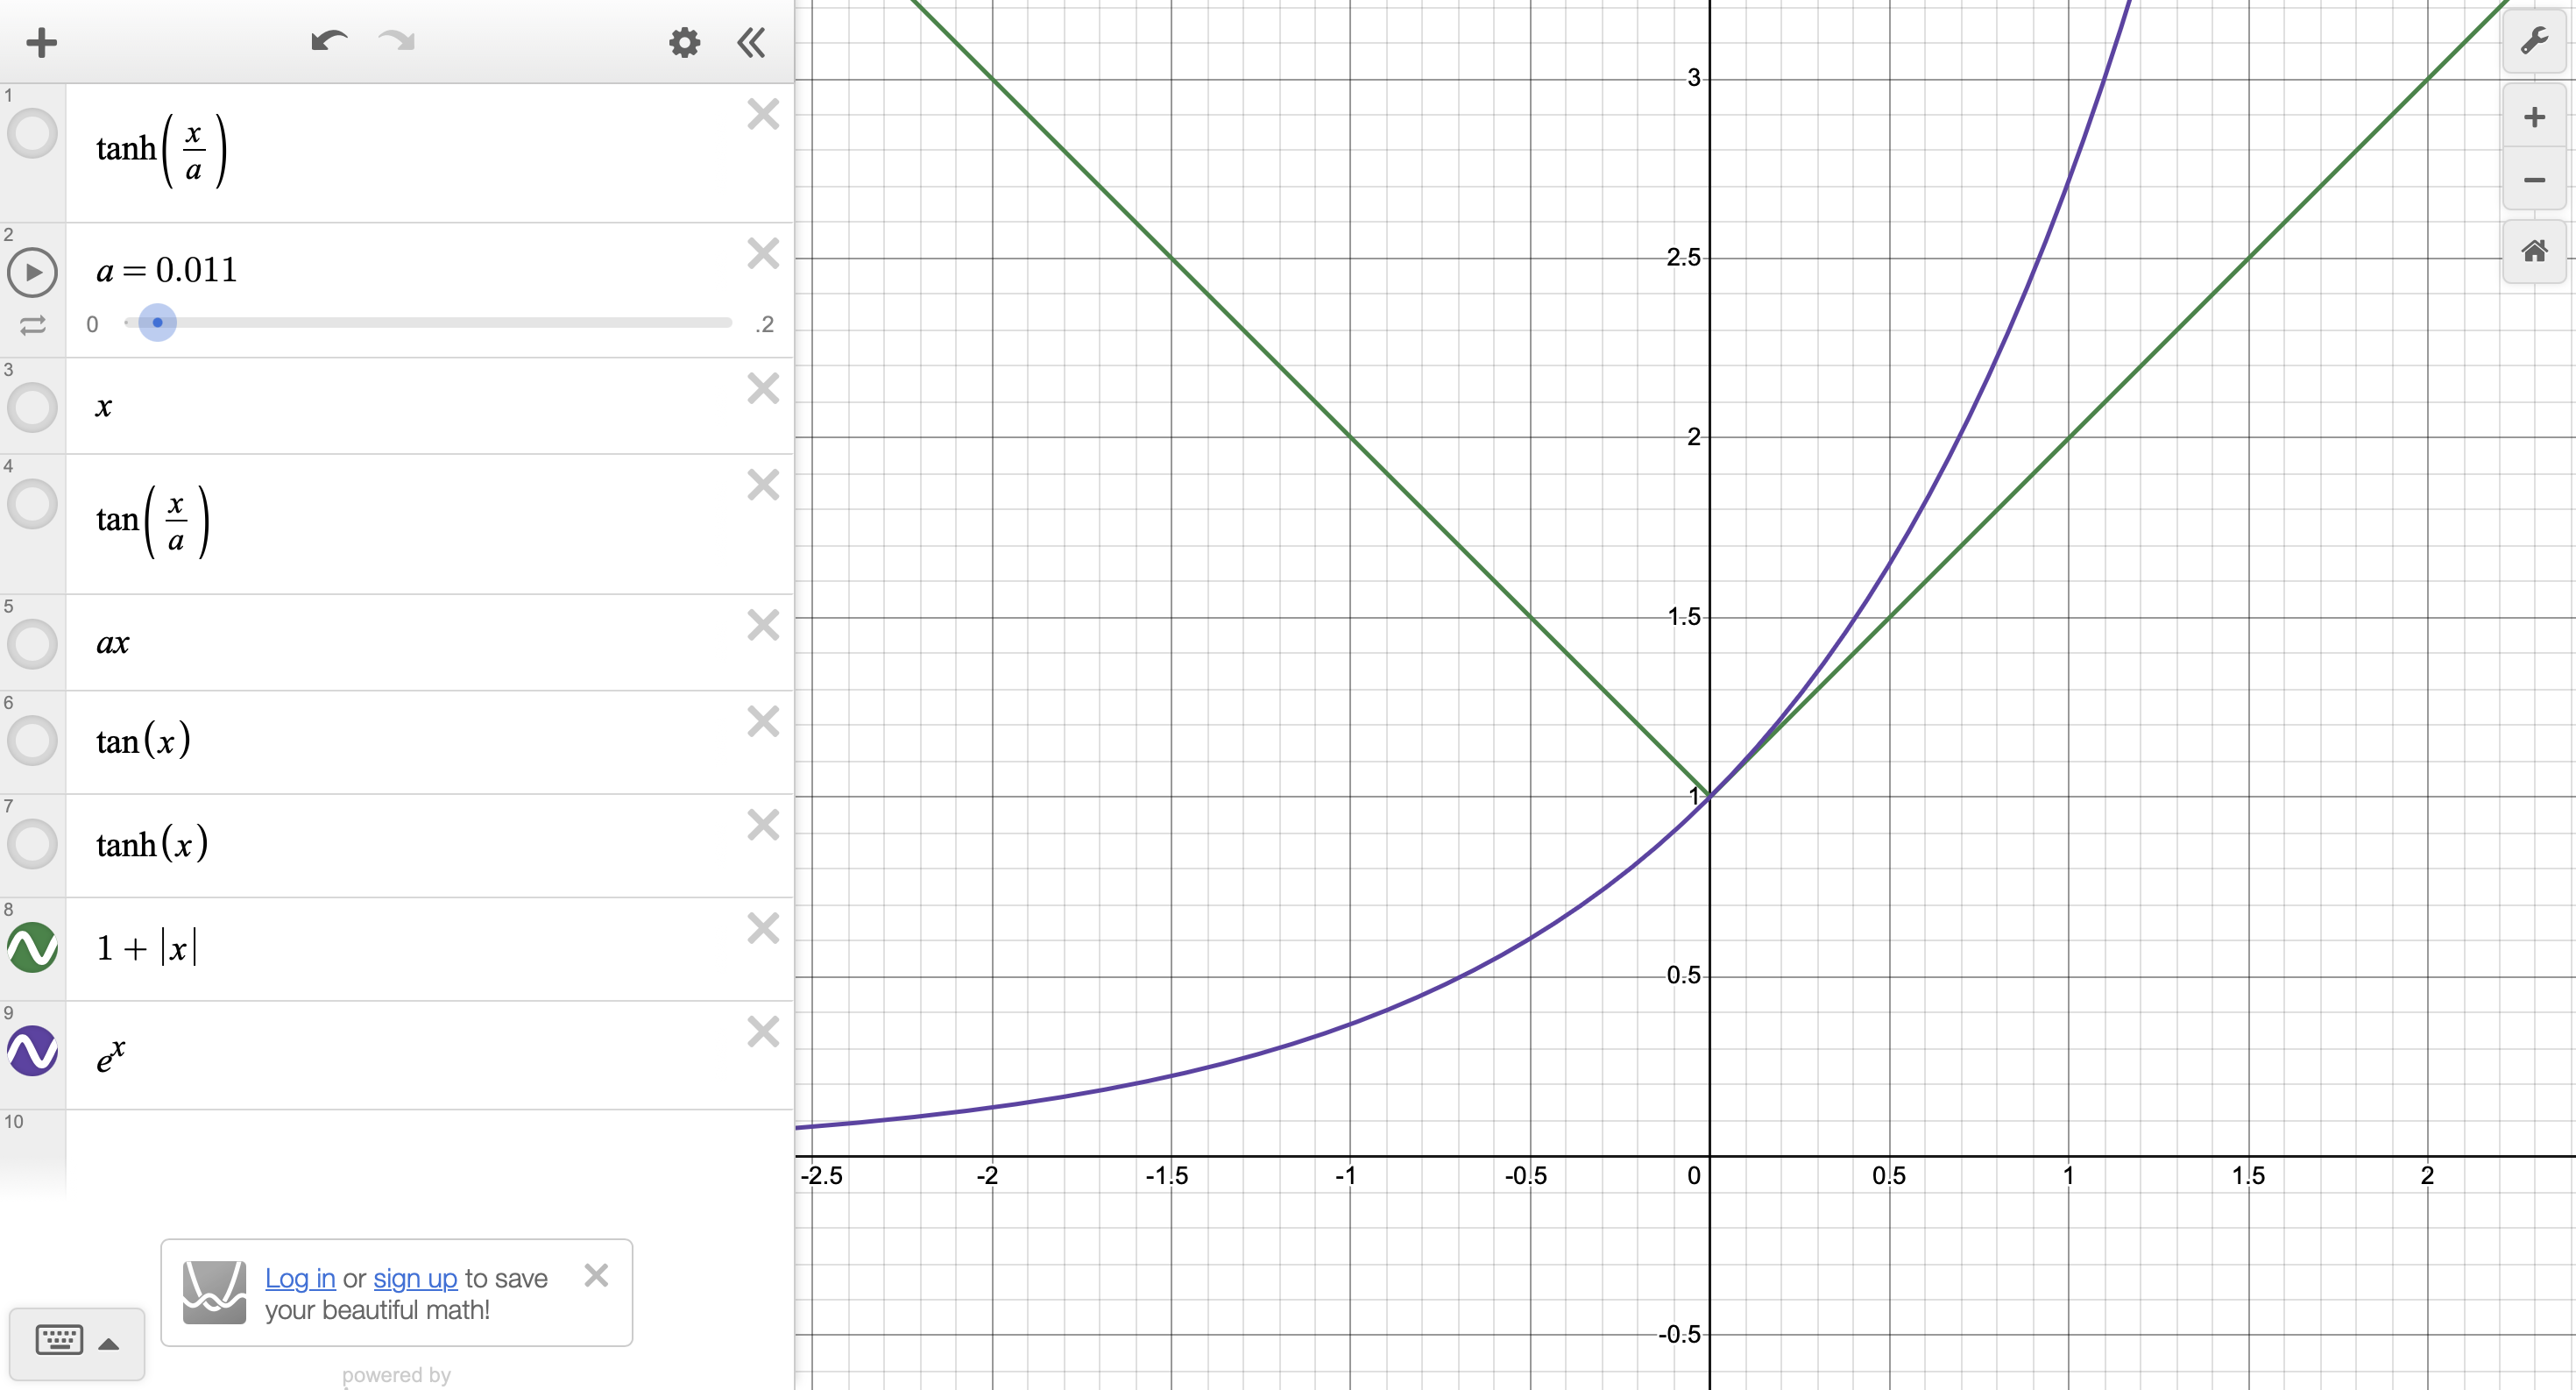
\includegraphics[width=.80\textwidth]{19.png}
      \end{center}
    \item It is helpful to rework the equation somewhat before attempting to
      find the asymptotic expansion. We can make the following simplification:
      \[ \vep = (e^x - 1)^2 - x^2 = (e^x - 1 - x)(e^x - 1 + x) \]
      Plugging in $x \sim a_1 \vep^\alpha$ gives
      \begin{align*}
        \vep & \sim \left(\frac{1}{2}a_1^2\vep^{2\alpha}\right)\left(2a_1\vep^\alpha\right) \\
        \vep & = a_1^3\vep^{3\alpha} \\
             & \Rightarrow \alpha = 1/3, a_1 = 1
      \end{align*}
      We can proceed with plugging in $x \sim \vep^{1/3} + a_2 \vep^\beta$, but
      first not that the left hand side can be expanded as follows:
      \[ (e^x - 1 - x)(e^x - 1 + x) = \left( \frac{x^2}{2} + \frac{x^3}{6} +
      \cdots \right)\left( 2x \frac{x^2}{2} + \cdots \right) = x^3 + x^4/3 +
    x^4/4 + \cdots = x^3 + \frac{7}{12}x^4 + \cdots \]

      This helps identify the next terms in the expansion:
      \begin{align*}
        0 & = 3a_2\vep^{2/3 + \beta} + \frac{7}{12}\vep^{4/3} \\
        \Rightarrow \beta & = 2/3, a_2 = -\frac{7}{36}
      \end{align*}
      So the asymptotic expansion is $x \sim \vep^{1/3} -
      \frac{7}{36}\vep^{2/3}$.
  \end{enumerate}
\end{solution}

\newpage
\begin{problem}[1.20]
  In this problem you should sketch the functions in each equation and then use this to determine
  the number and approximate location of the real-valued solutions. With this, find a three-term
  asymptotic expansion, for small $\vep$, of the nonzero solutions.
  \begin{enumerate}
    \item $x = \tanh \left(\frac{x}{\vep}\right)$,
    \item $x = \tan\left(\frac{x}{\vep}\right)$.
  \end{enumerate}
\end{problem}

\begin{solution}
  \begin{enumerate}
    \item 
      The function $\tanh(x/\vep)$ has two roots away from 0 as shown in the
      included Figure $\ref{fig:20tanh}$. To find an expansion for this, we make
      the change of variables $y = x/\vep$ and get $\vep y = \tanh y$. Then we
      can assume that $y = \lambda + r$ with $\lambda \gg 1$ and $r \ll
      \lambda$ (Solutions are large after making the transformation). Plugging
      this in gives
      \begin{align*}
        \vep\lambda + \vep r & = \tanh(\lambda + r) \\
                             & = \frac{e^{2(\lambda + r)} - 1}{e^{2(\lambda +
        r)} + 1} \\
                             & = 1 - \frac{2}{e^{2(\lambda + r)} + 1} \\
      \end{align*}
      For $\lambda \gg 1$, we get $\vep\lambda = 1 \Rightarrow \lambda =
      \vep^{-1}$. Now we check the next order:
      \begin{align*}
        \vep r & \sim -\frac{2}{e^{2(\lambda + r)} + 1} \\
               & \sim -2e^{-2r}e^{-2/\vep} \\
               & \sim -2e^{-2/\vep} \\
        \Rightarrow y & \sim \vep^{-1} -2\vep^{-1}e^{-2/\vep} \\
        \Rightarrow x_r & \sim 1 -2e^{-2/\vep}
      \end{align*}
      By symmetry, we can also find the other root $x_l \sim -1 + 2e^{-2/\vep}$.
    \item 
      The function $\tan(x/\vep)$ has an infinite number of  roots away from 0
      as shown in the included Figure $\ref{fig:20tan}$. To find an expansion
      for this, we make the same change of variables to get $\vep y = \tan(y)$.
      Then we guess that $y = a_0 + a_1\vep^\alpha$, but we can observe that
      $a_0 = n\pi$ for $n \in \mathbb{Z}$. Plugging this in gives
      \[ \vep n \pi = \tan(n\pi + a_1\vep^\alpha) = \tan(a_1\vep^\alpha) \sim
      a_1\vep^\alpha. \]
      So $\alpha = 1, a_1 = n\pi$. Now we can check the next order:
      \[ \vep n \pi = \tan(n\pi + \vep n \pi + a_2 \vep^\beta) \sim
      a_2\vep^\beta \]
      \( \Rightarrow \beta = 2, a_2 = n\pi^2/3 \) and we get $y \sim n\pi(1 +
      \vep + \vep^2)$, $x \sim n\pi(\vep + \vep^2 + \vep^3)$.
  \end{enumerate}

  \begin{figure}
    \centering
    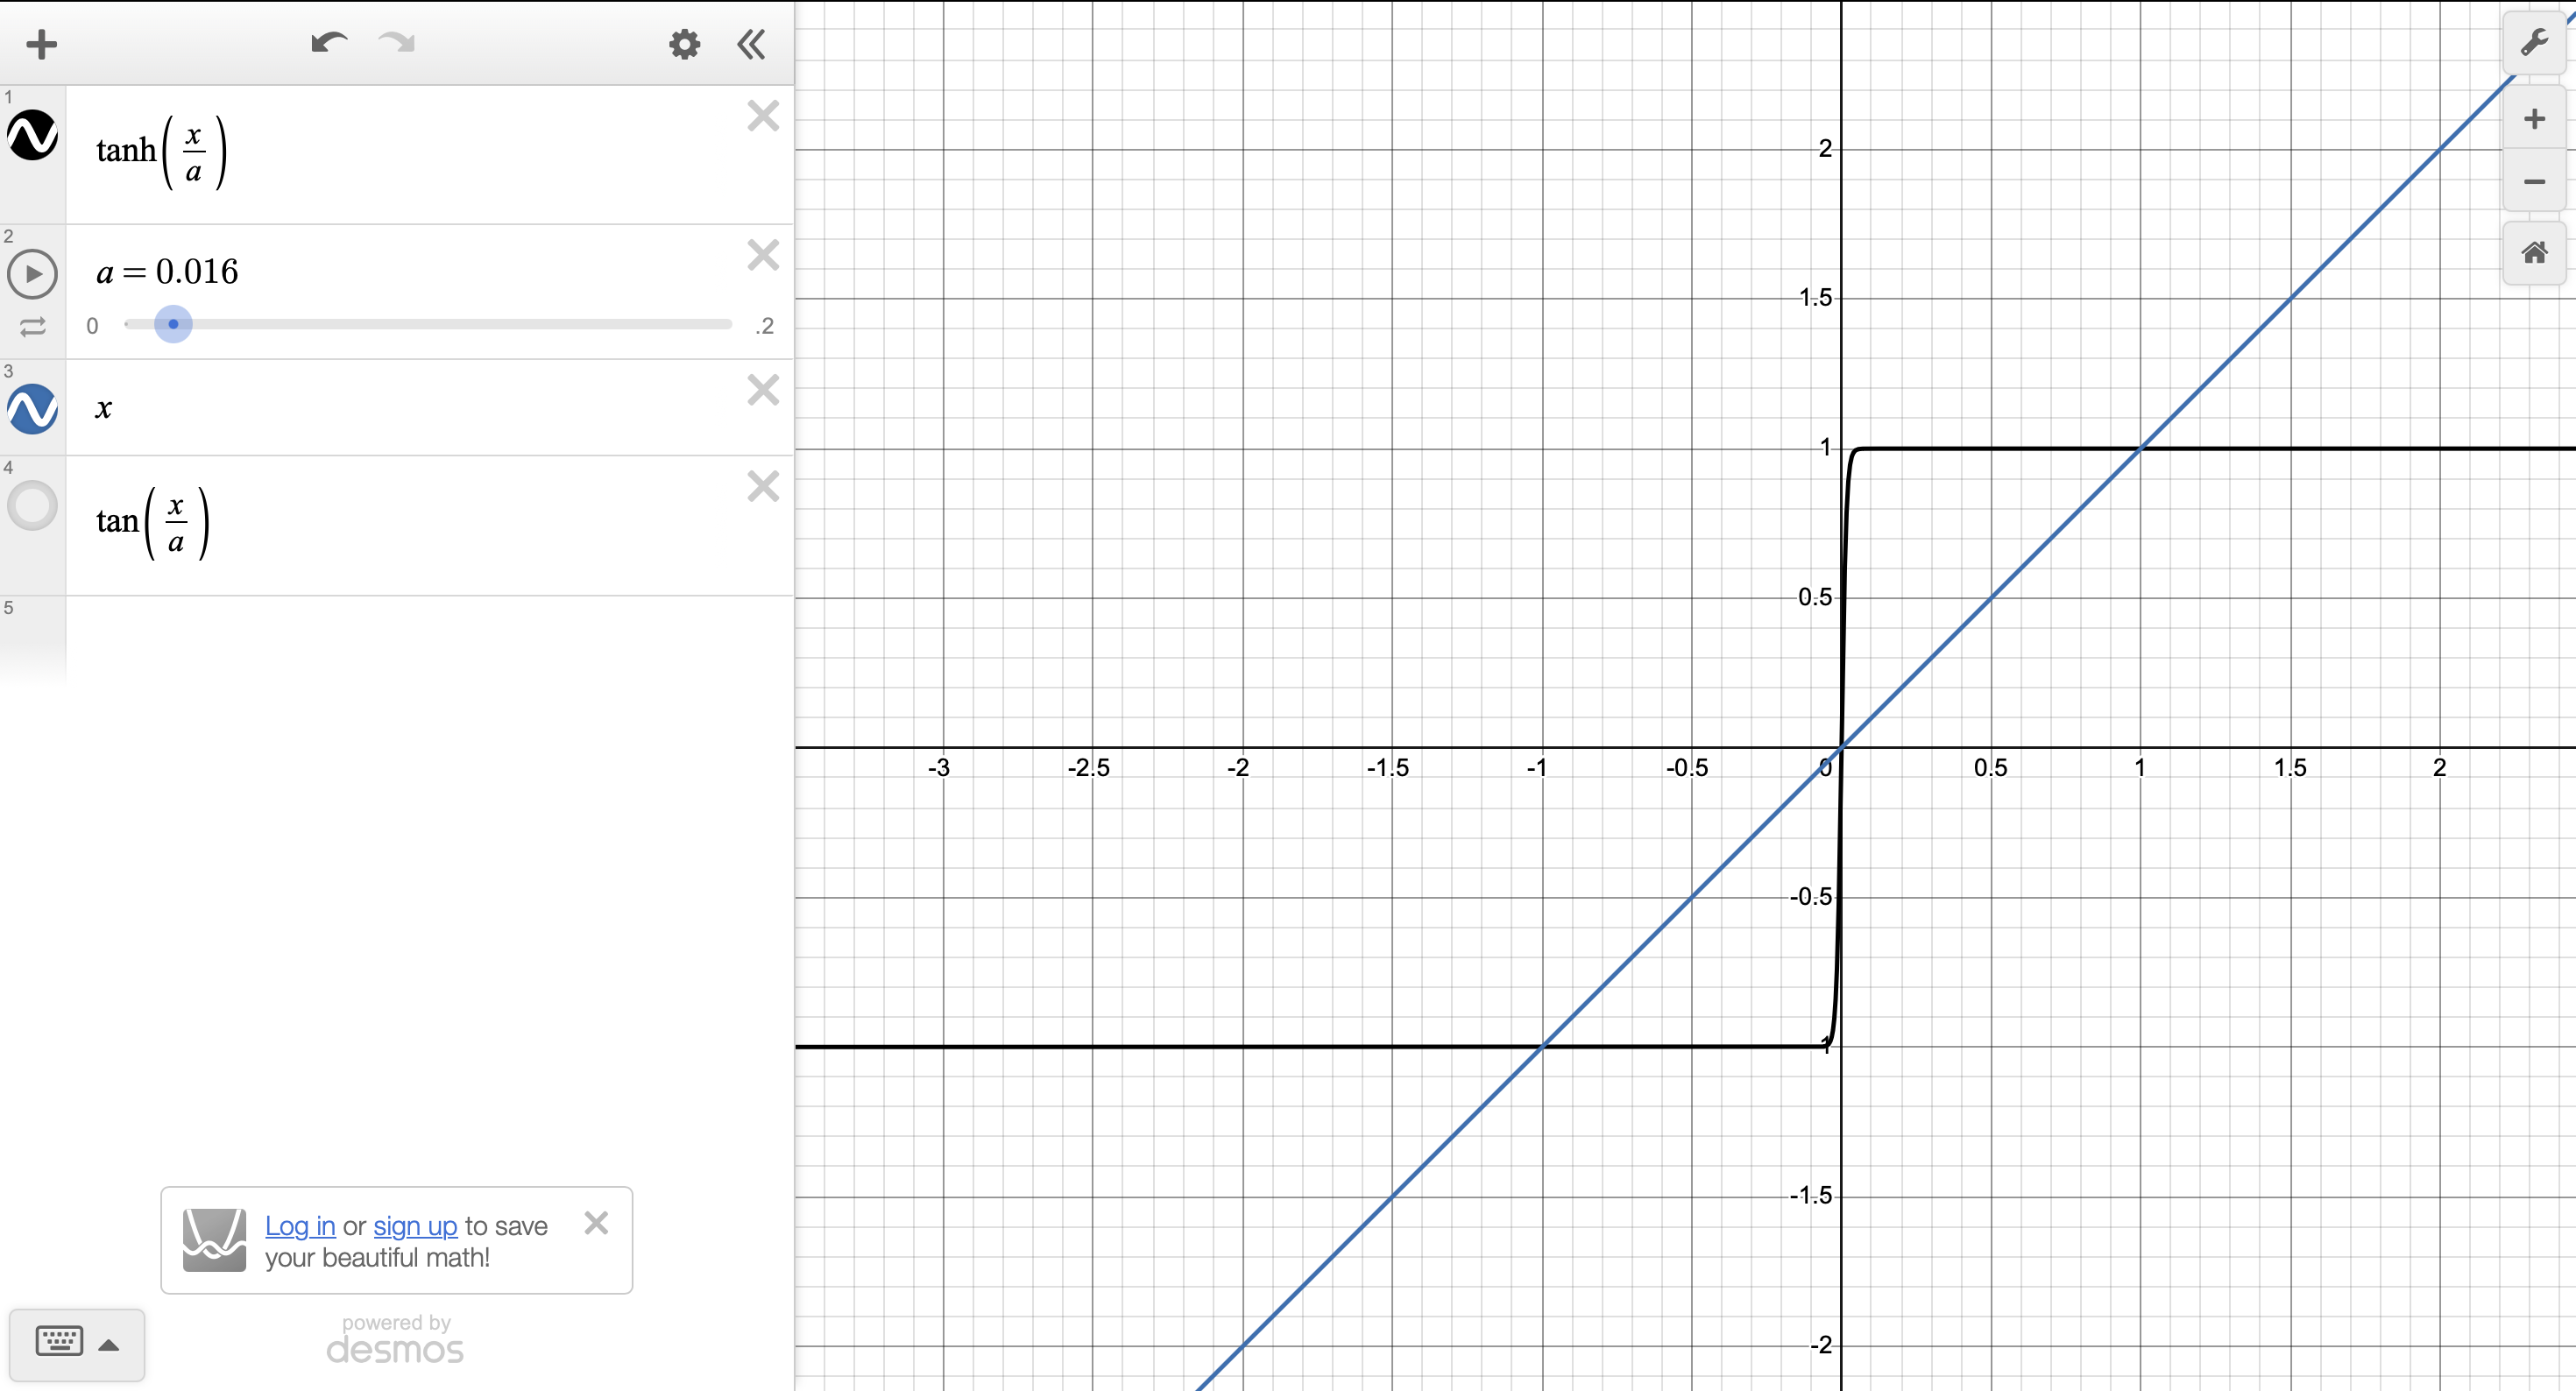
\includegraphics[width=0.8\textwidth]{20_tanh.png}
    \caption{Graph of $\tanh(x/\vep)$ and $x$}
    \label{fig:20tanh}
  \end{figure}
  \begin{figure}
    \centering
    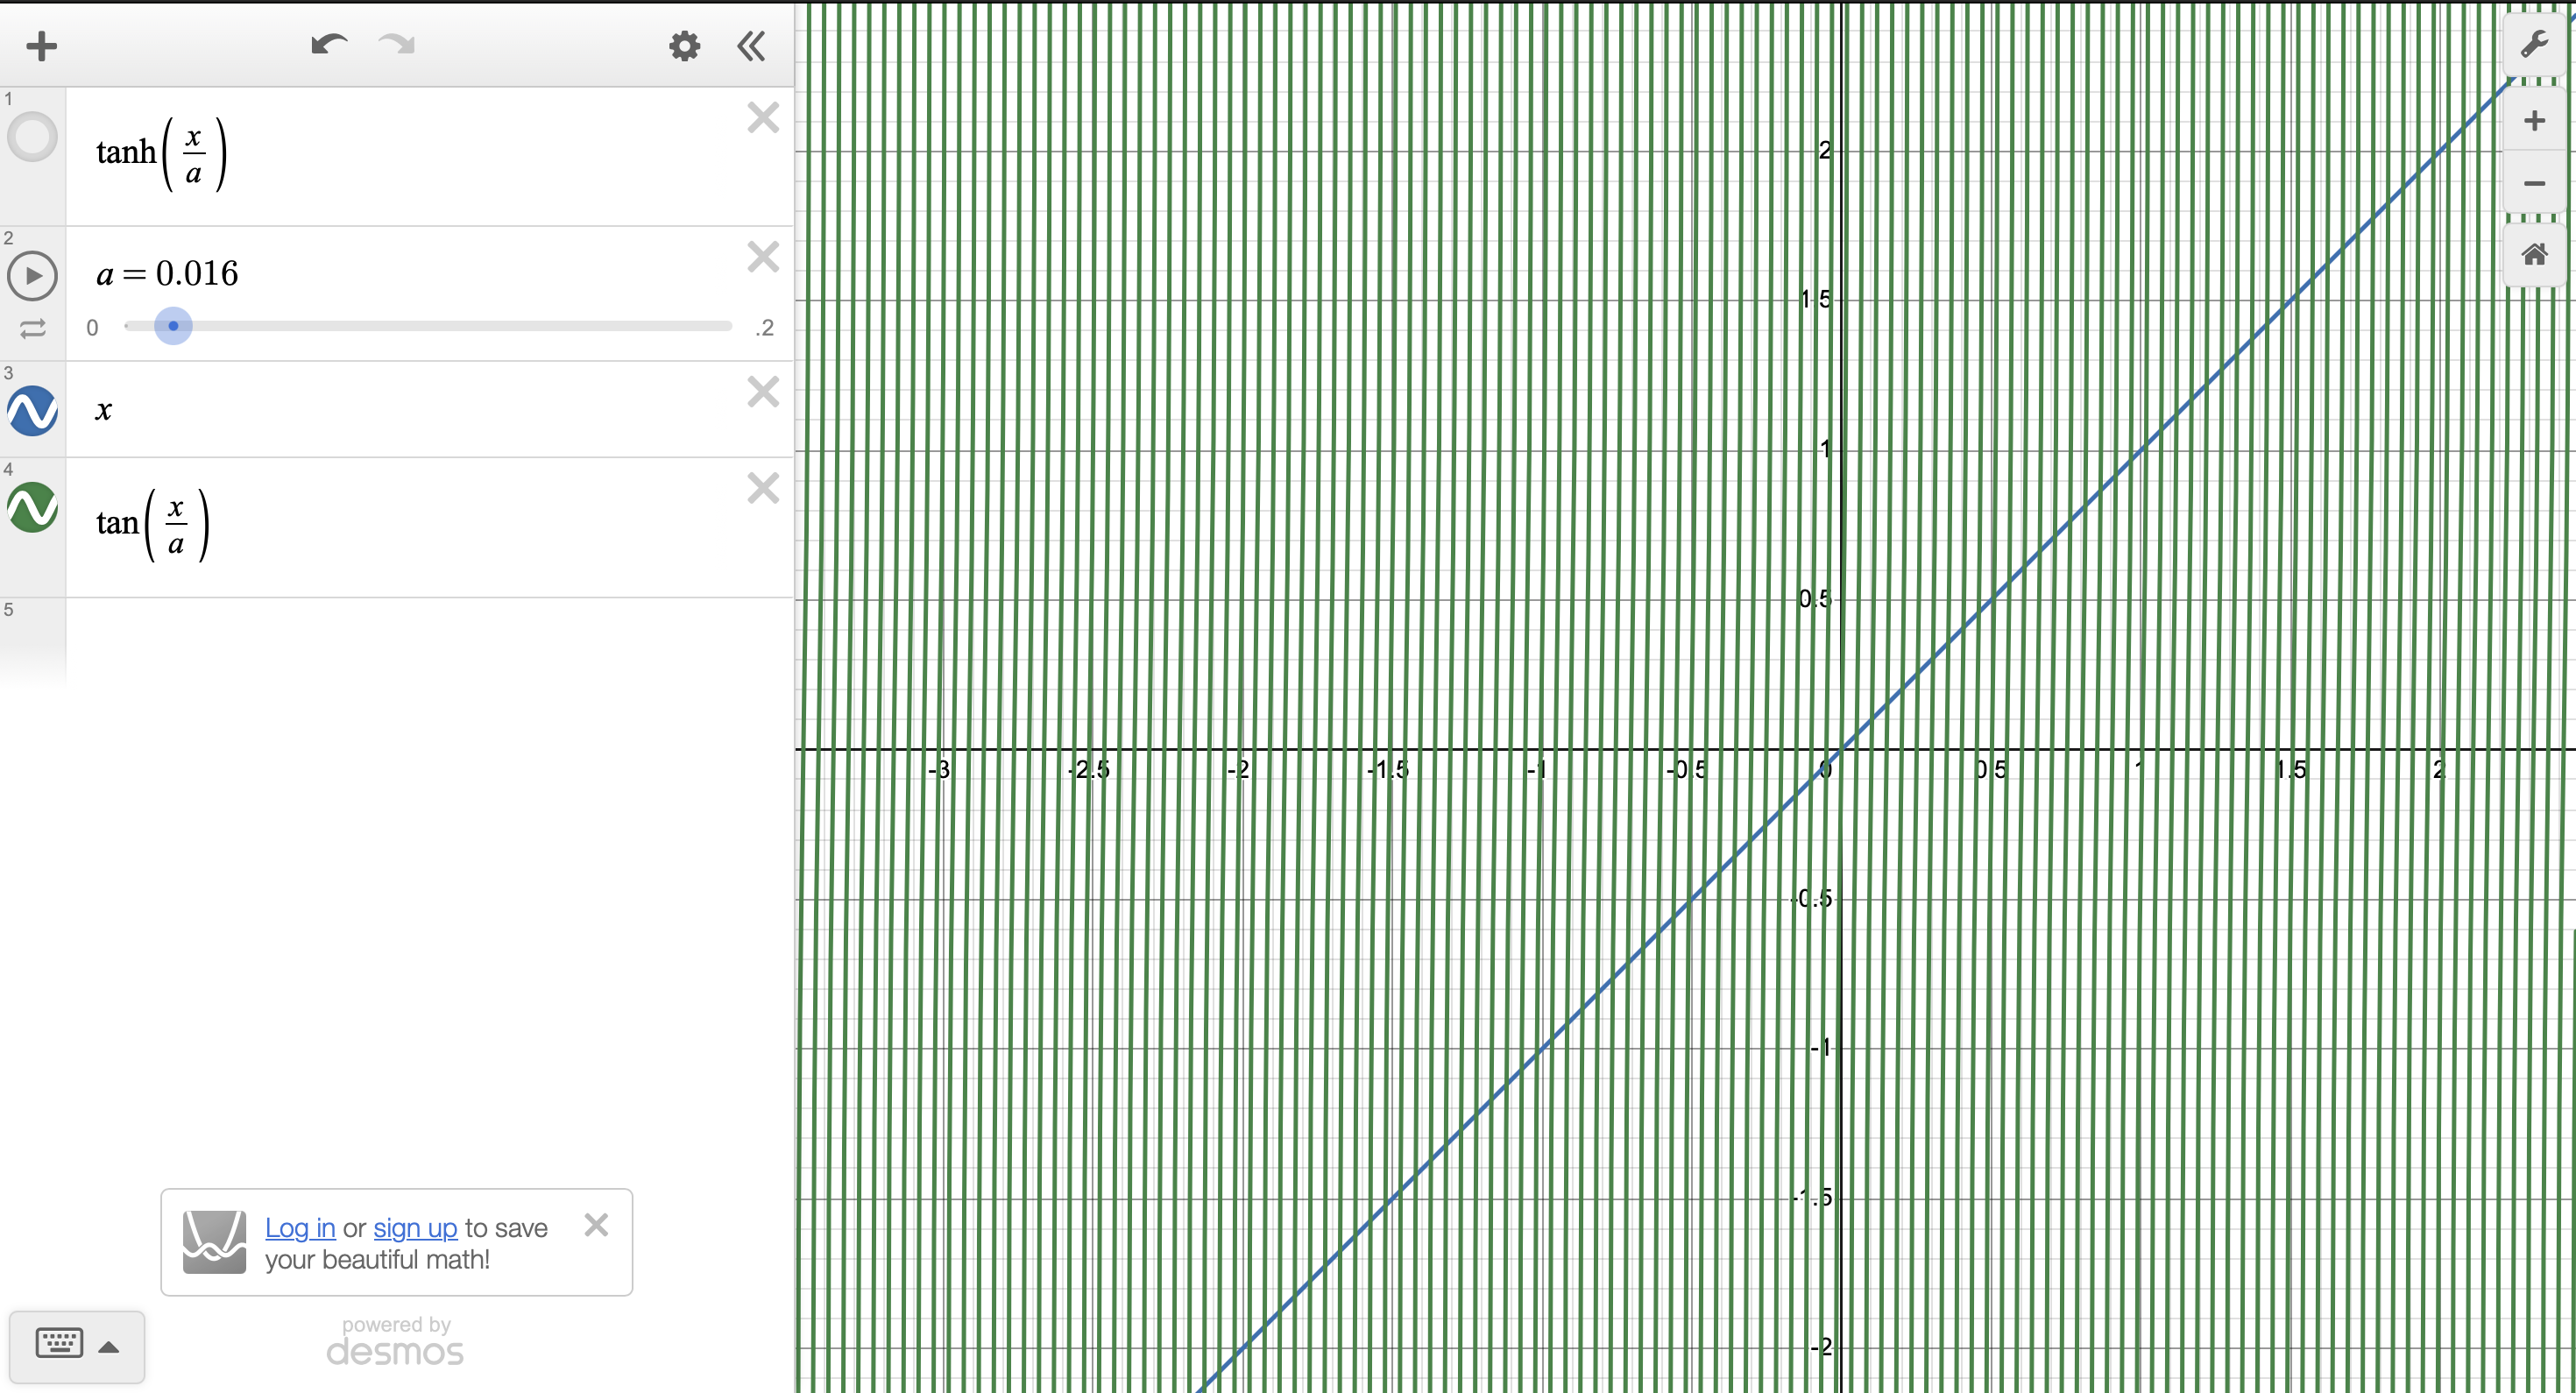
\includegraphics[width=.8\textwidth]{20_tan.png}
    \caption{Graph of $\tan(x/\vep)$ and $x$}
    \label{fig:20tan}
  \end{figure}
\end{solution}

\newpage
\begin{problem}[1.21]
  To determine the natural frequencies of an elastic string, one is faced with solving the equation
  $\tan(\lambda) = \lambda$.
  \begin{enumerate}
    \item After sketching the two functions in this equation on the same graph explain why there is
      an infinite number of solutions.
    \item To find an asymptotic expansion of the large solutions of the equation, assume that
      $\lambda \sim \vep^{-\alpha}(\lambda_0 + \vep^\beta\lambda_1$. Find
      $\vep, \alpha, \beta, \lambda_0, \lambda_1$ (note that $\lambda_0$ and $\lambda_1$ are
      nonzero and $\beta > 0$).
  \end{enumerate}
\end{problem}

\begin{solution}
  \begin{enumerate}
    \item As can be seen in Figure \ref{fig:21}, since $\tan(x)$ is periodic and has
      full range, there are infinitely many solutions to the equation since the
      line $y = \lambda$ will cross each branch of the $\tan(x)$ function. The
      crossing points for large $\lambda$ will be close to the vertical asymptotes
      of the tangent function at $\lambda_k = \frac{1}{2}(2k-1)\pi$ for $k \in \mathbb{Z}$.
      \begin{center}
        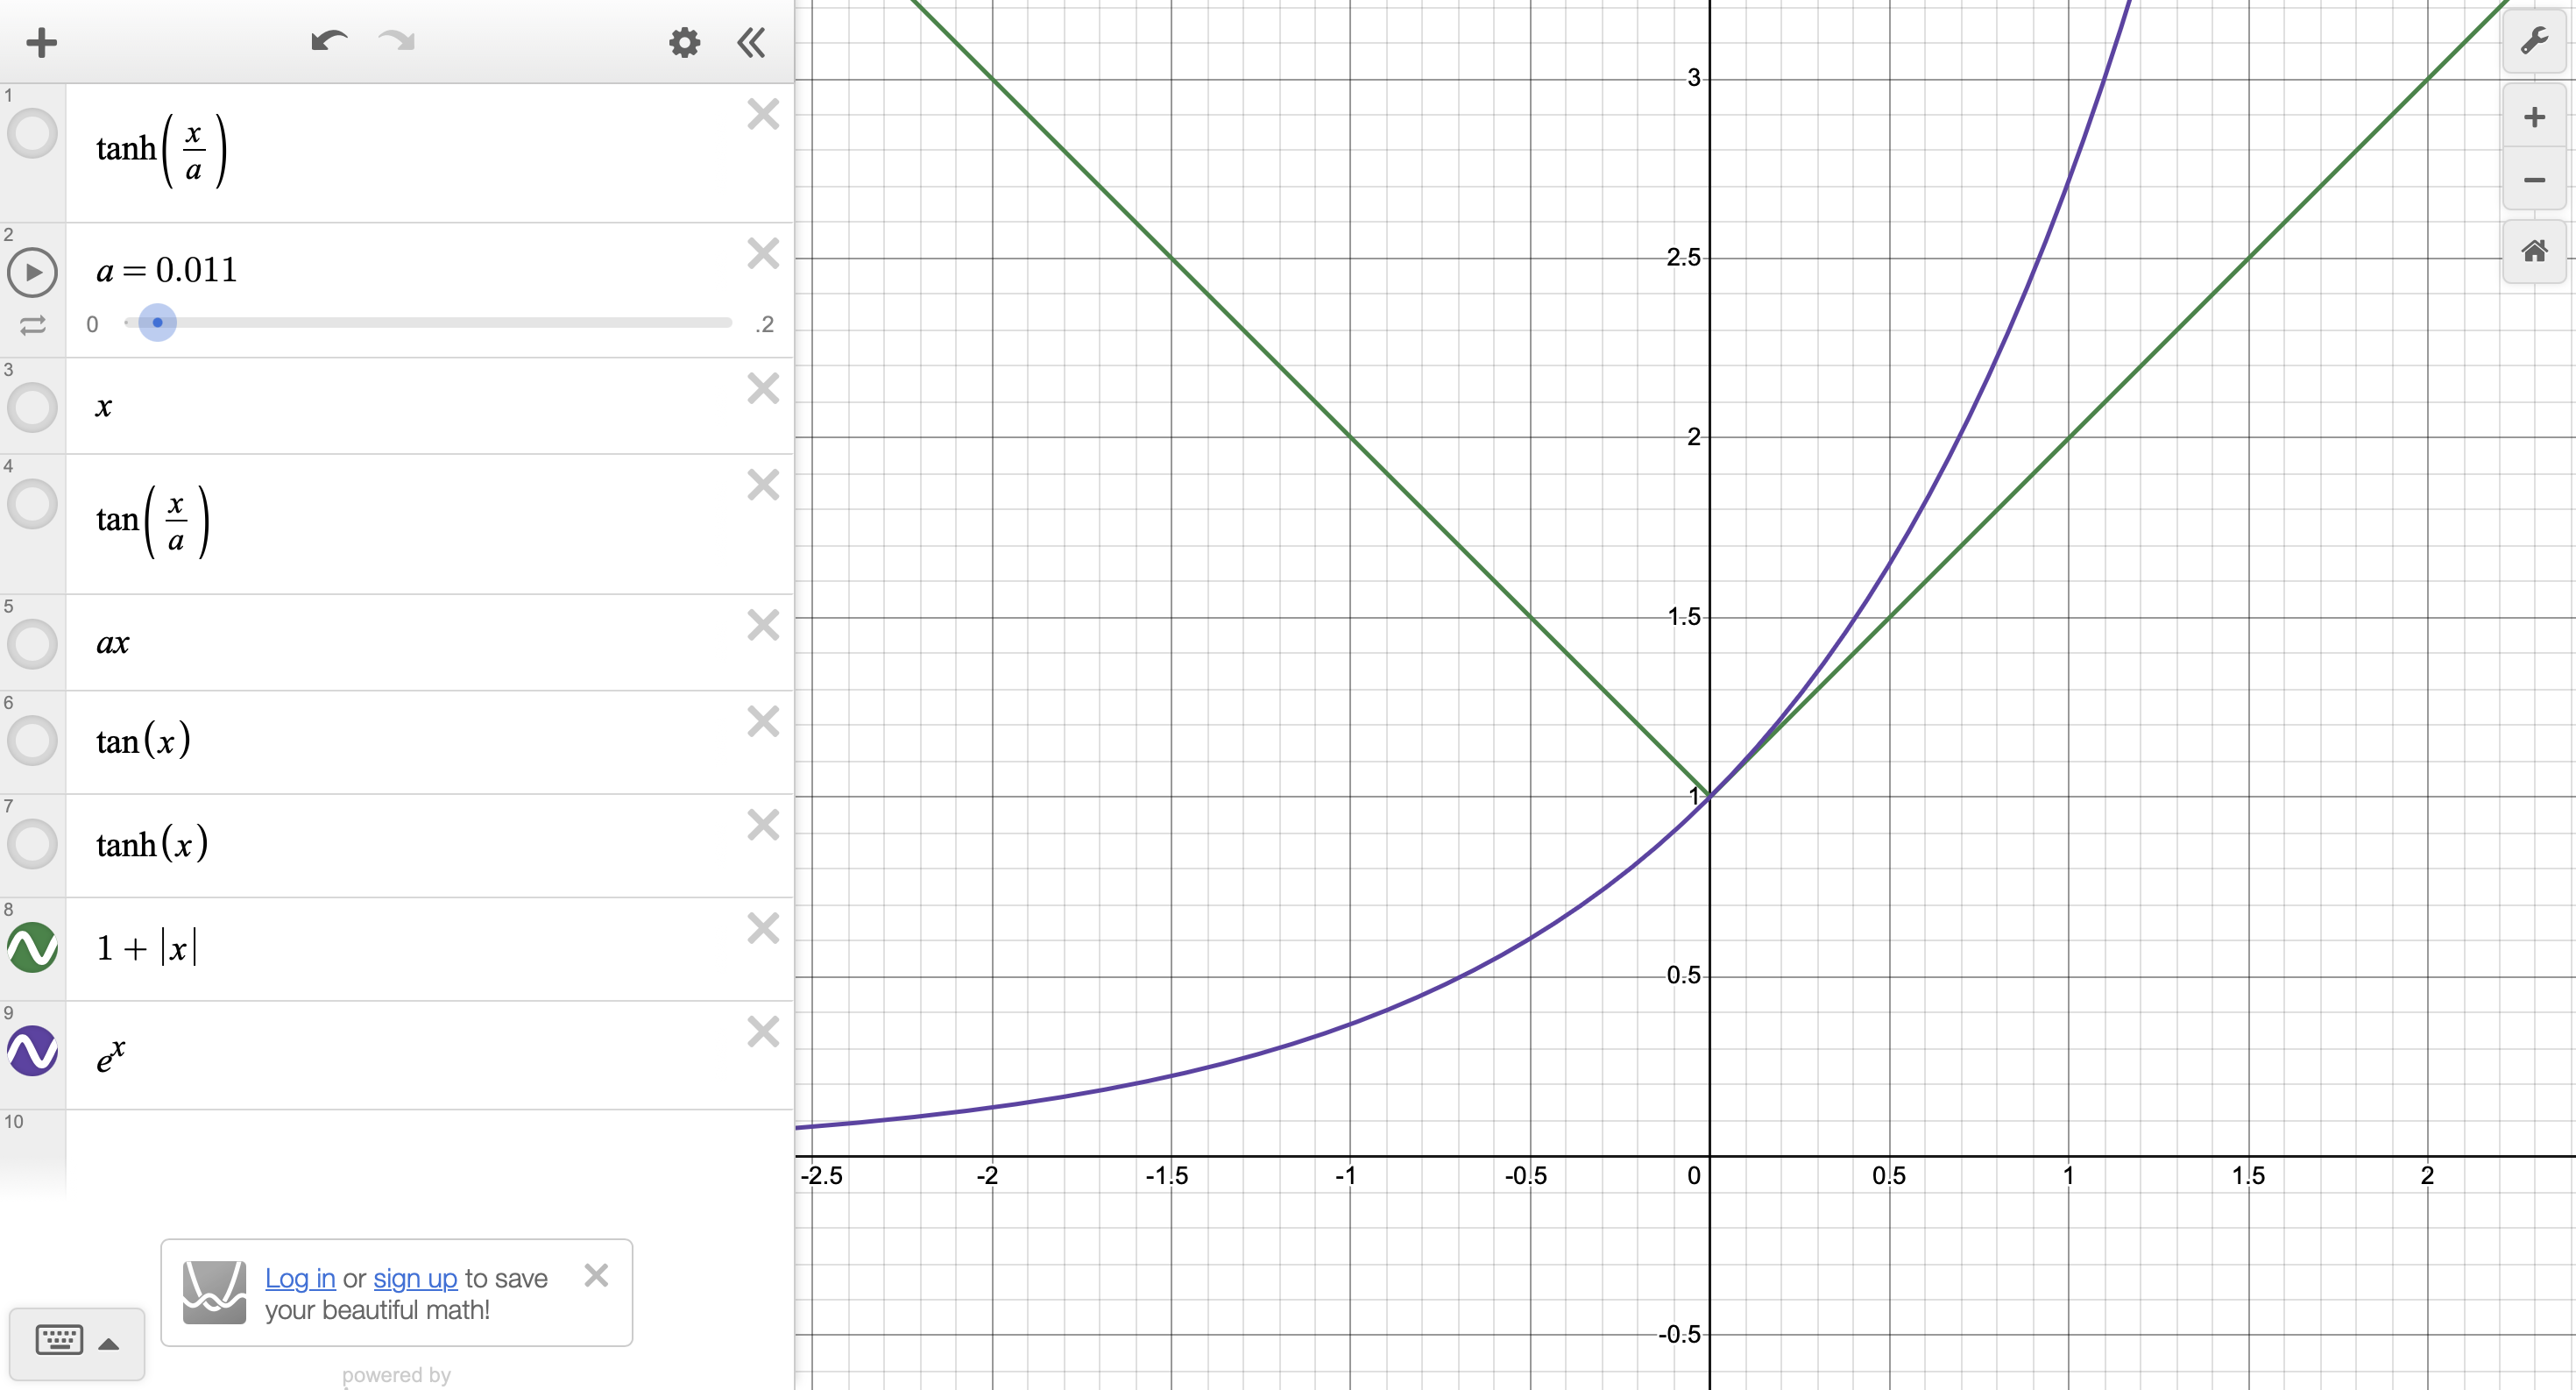
\includegraphics[width=.80\textwidth]{19.png}
        \label{fig:21}
      \end{center}
    \item For values of $\lambda$ near $\lambda_k$, we can expand sine and
      cosine to get
      \begin{align*}
        \sin(\lambda) & \sim 1 - \frac{1}{2}(\lambda - \lambda_k)^2 \\
        \cos(\lambda) & \sim 0 - (\lambda - \lambda_k) + \frac{1}{6}(\lambda -
          \lambda_k)^3 \\
        \Rightarrow \tan(\lambda) & \sim \frac{1 - \frac{1}{2}(\lambda -
          \lambda_k)^2}{-(\lambda - \lambda_k) + \frac{1}{6}(\lambda -
          \lambda_k)^3} \\
            & \sim -\frac{1}{\lambda - \lambda_k} \cdot \frac{1 - \frac{1}{2}(\lambda
              - \lambda_k)^2}{1 - \frac{1}{6}(\lambda -
              \lambda_k)^2} \\
            & \sim -\frac{1}{\lambda - \lambda_k} \left[ 1 - \frac{1}{3}(\lambda -
              \lambda_k)^2 \right] \\
      \end{align*}
      For large solutions, we know from the picture that $\lambda \sim
      \lambda_k$, so we can assume $\lambda \sim \lambda_k + \mu$ where $\mu \ll
      \lambda_k$. Then the previous calculation gives 
      \begin{align*}
        \lambda_k + \mu \sim \frac{-1}{\mu} & \sim (1 - \frac{1}{3}\mu^2) \\
        \lambda_k\mu + \mu^2 & \sim -1 + \frac{1}{3}\mu^2 \\
      \end{align*}
      which, after dropping higher order terms, implies that $\mu =
      -\frac{1}{\lambda_k}$. Therefore, we have the asymptotic expansion up to
      two terms $\lambda \sim \lambda_k - \frac{1}{\lambda_k}$.


  \end{enumerate}
\end{solution}

\end{document}

